\section{The Big Idea}
 \begin{wrapfigure}{r}{0.25\columnwidth}
		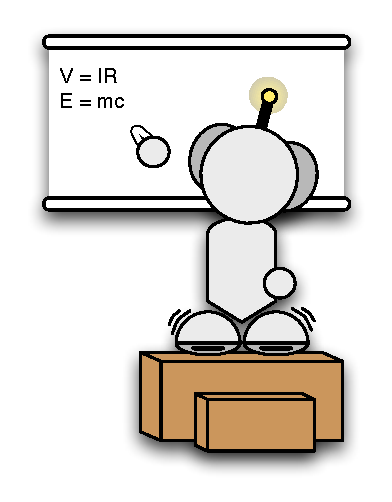
\includegraphics[width=0.25\columnwidth, trim=10mm 10mm 10mm 10mm]{diagrams/robot_whiteboard.pdf}
 \end{wrapfigure}
We propose the following offline strategy for identifying and \textbf{eliminating
symmetric paths} in 4-connected grid maps:
\begin{enumerate}
\item{Decompose the grid map into a set of empty rectangular rooms.}
\item{Prune all tiles not on the perimeter of an empty room.}
\item{Connect tiles on opposite sides of the perimeter.}
\end{enumerate}
Sometimes a tile which has been pruned is later required; for example as a start
or goal location. 
We handle these cases by temporarily re-inserting the 
required tile back into the grid map for the duration of the search.

\begin{figure}[t]
\begin{minipage}{18in}
\label{fig:splash}
\begin{center}
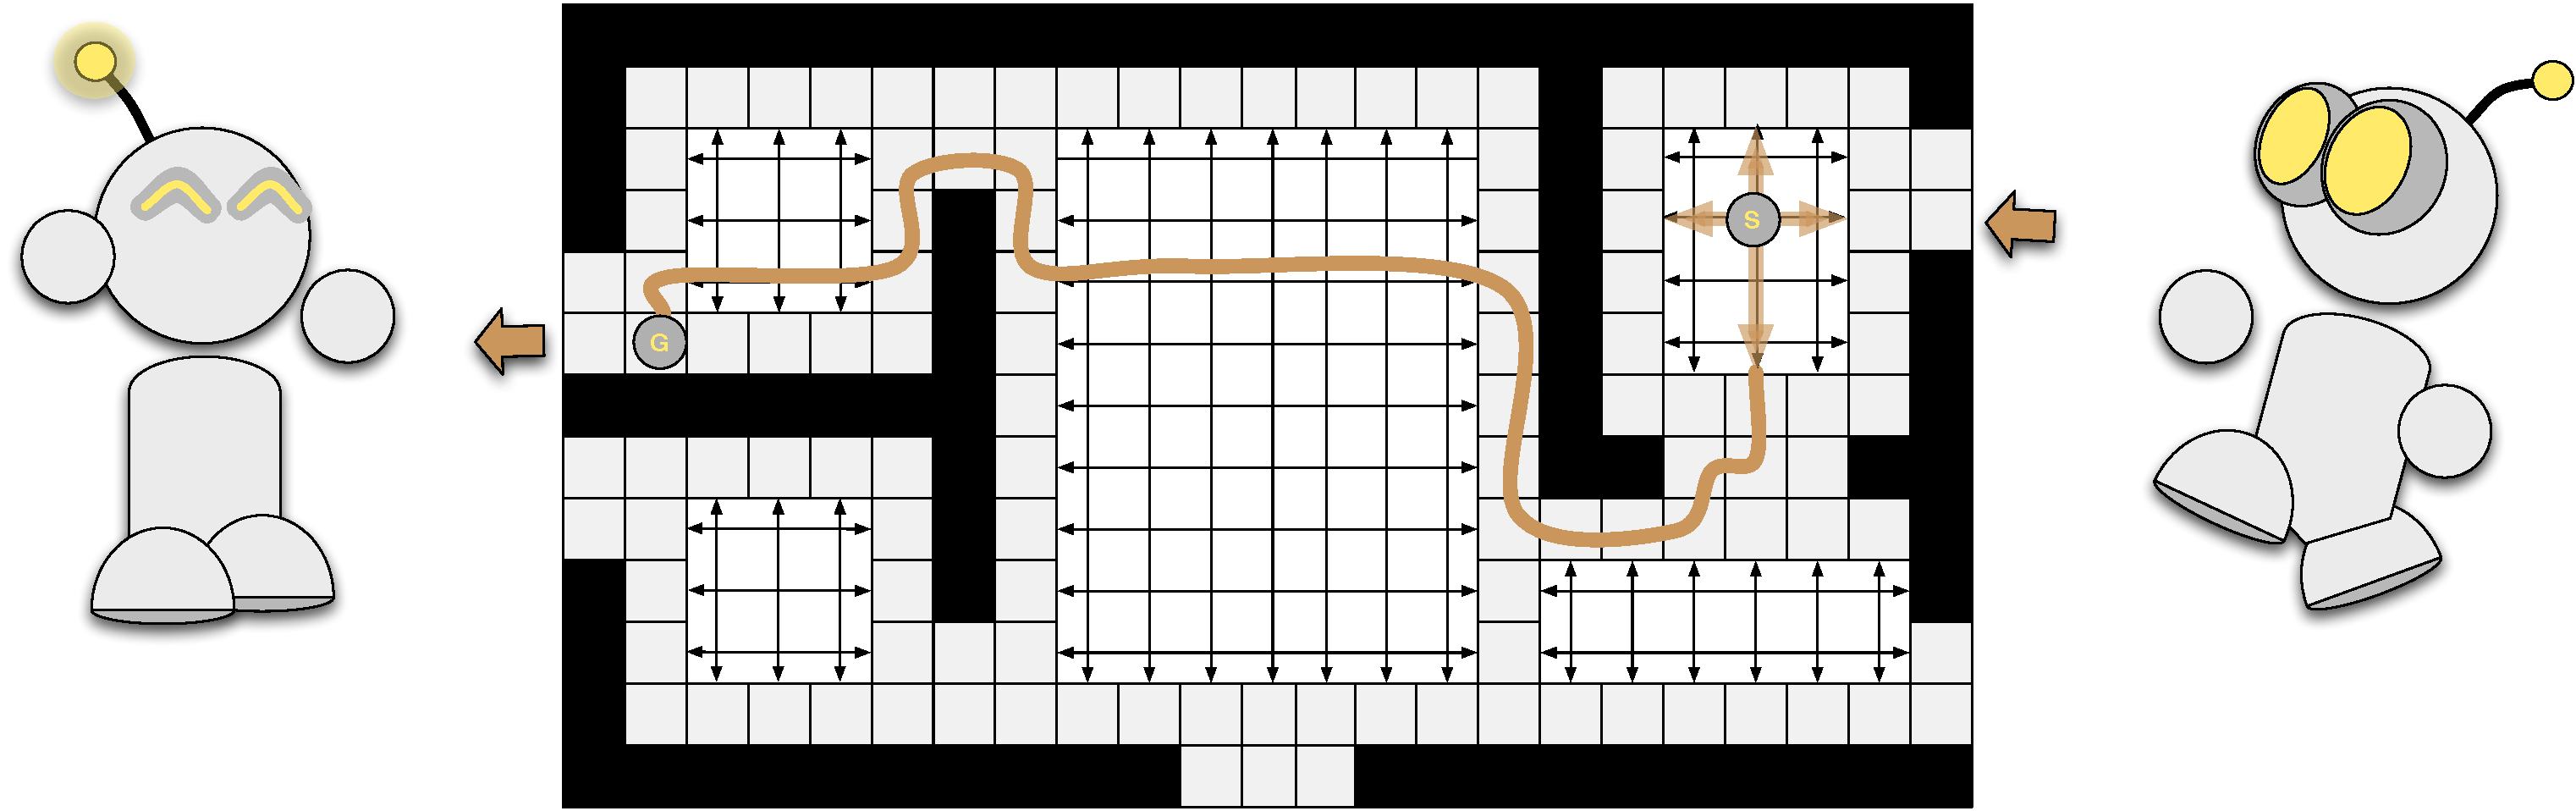
\includegraphics[width=18in]{diagrams/robot_splash2}
\caption{We speed up search by decomposing a 4-connected map into rectangular
rooms which can be traversed without visiting any tiles from their interior.} 
\end{center}
\end{minipage}
\vspace{2em}
\end{figure}
